
\label{sec:visualDomain}
	

\subsubsection{LightSource und LightSourceManager}
	
	\lstinline|LightSourceManager| ist eine Singleton-Klasse, welche sämtliche 
	\lstinline|LightSource|-Instanzen erstellt, besitzt und verwaltet. Sie erstellt, besitzt
	und updatet die Uniform Buffers, welche die GLSL-LightSource-Structures für die Beleuchtungs-Berechnungen
	im Fragment Shader enthalten. Dasselbe gilt für den Uniform Buffer, der im Falle von Layered Rendering
	die Shadowmap-Lookup-Matrizen enthält. Da sich die Buffer-Inhalte durch Transformationen oder Änderungen
	anderer Eigenschaften wie Farbe oder Spot Light-Öffnungswinkel immer ändern können, ruft 
	\lstinline|LightingSimulator::stepSimulation()| die Update-Routine jeden Frame auf.
	Die \lstinline|Shader|-Klasse bezieht die Uniform Buffers bei Bedarf von \lstinline|LightSourceManager|,
	um sie an die entsprechenden Uniform-Variablen in Shader-Programm zu binden.\\
	
	\lstinline|LightSource| ist die abtrakte Basisklasse für \lstinline|PointLight| und \lstinline|SpotLight|.
	Sie erbt für etwaige Visualisierungszwecke von \lstinline|WorldObject|. Sie gibt Auskunft darüber, ob es sich
	um einen Shadow Caster handelt und/oder ob die Lichtquelle gerade aktiviert ist.
	\lstinline|PointLight| und \lstinline|SpotLight| haben Convenience Functions, um Matrizen für Shadowmap-
	Generierung oder -Lookup bereit zu stellen, z.B.:
	 
	\begin{lstlisting}
//matrix for shadowmap lookup in VIEW space: bias*perspLight*viewLight * (camView)^-1 ;
//returns getBiasedViewProjectionMatrix(scale,translation) * spectatorCam->getViewMatrix().inverse();
//scale is configurable in case one wants to use rectangle texture for whatever reason...
Matrix4x4 getViewSpaceShadowMapLookupMatrix( Camera* spectatorCam,
	float scale= 0.5f, float translation= 0.5f);
	\end{lstlisting}
	 
	Die Structure, die die Lichtquellen für GLSL definiert, ist generisch, d.h. sowohl Point als auch Spot Lights
	sind in ihr codierbar. Die Identifikation als Point Light geschieht darüber, dass alle ausschließlich 
	Spot Light-relevanten Werte null sind. Dieser nicht ganz saubere Mechanismus ist nötig, da
	\begin{enumerate}
		\item GLSL keine Vererbung kennt und
	 	\item die Assotiation zwischen Buffer-Members und Refererenzierung einzelner Members im Shader sich sonst
	 		 unnötig verkomplizieren würde (s. Abschnitt \ref{sec:uniformBuffers})
	\end{enumerate}
	. Außerdem sollte zunächst kein anderer Basis-Datentyp als \lstinline|float| in der Structure enthalten sein,
	da Treiber-Bugs vor allem bei modernen Features auftauchen, und erst einmal eine funktionsfähige Implementation 	
	existieren sollte. Deshalb wurde keine \lstinline|bool|- oder \lstinline|int|-Variable zur Lichtquellen-Typ-	
	Unterscheidung benutzt. Jede GLSL-LightSource ist außerdem über sein Shadowmap-Layer als Shadow-Caster identifizierbar.
	Ein Wert von -1 oder größer als der maximalen Anzahl Shadow Caster zeigt an, dass die Quelle keine assoziierte
	Shadowmap hat. Auf diese Weise wird die Reihenfolge im Buffer entkoppelt von der Funktion als Shadow-Caster.
	Dies könnte sinnvoll sein in einem Kontext, wo nur eine bestimmte Anzahl an Lichtquellen von der Anwendungslogik
	dynamisch nach einer bestimmte Metrik (z.B. Nähe zur Betracher-Kamera, Helligkeit) als Shadow-Caster getaggt werden.
	
\subsubsection{RenderTarget}	
	Das \lstinline|RenderTarget| abstrahiert nicht nur das OpenGL Frame Buffer Object (FBO), sondern optional
	auch als Container für eine Sammlung an Texturen mit unterschiedlicher Semantik. Auf diese Weise kann z.B. 
	eine Instanz dieser Klasse beim Deferred Rendering direkt als G-Buffer verwendet und durch die einzelnen
	involvierten Simulations-Stages gereicht werden. Es existieren sowohl Member-Variablen für gerade angehängte
	Texturen, als auch welche für "`besessene"' Texturen. So können beliebig Texturen für Zwischen-Ergebnisse an-
	und ausgehängt werden, ohne die Besitzverhältnisse durcheinander zu bringen.
	


\subsubsection{genutzte moderne OpenGL- Features}	
	\label{sec:usedOpenGLfeatures}

	\paragraph{Hintergrund: Batching}
	Durch zunehmende Parallelisierung steigt die Rechenleistung vor allem von Graphikkarten ständig an.
	Hierdurch wird es möglich, immer komplexere Simulationen in Echtzeit durchzuführen.
	Was jedoch nicht in gleichem Maße ansteigt bzw. abnimmt, ist die Speicher-Bandbreite bzw. -Latenz.
	Hiermit wird der Faktor Datentransfers immer mehr zum Flaschenhals. Da mit jedem API-Call ein
	Overhead verbunden ist, ist es nötig, ihre Anzahl so gering wie möglich zu halten.
	Das bekannteste und kristischste Beispiel für einen solchen Overhead ist der Immediate Mode in OpenGL, 
	wo man Vertex-Attribute definiert, in dem man -- jeden Frame aufs neue -- 
	pro Vertex und pro Attribut einen API-Call ausführt:
	
	\begin{lstlisting}
glBegin(GL_TRIANGLES);
for(int i = 0; i<mVertices.size();i++){
	glVertex3f(mVertices[i].x,mVertices[i].y,mVertices[i].z);
	glNormal3f(mNormals[i].x,mNormals[i].y,mNormals[i].z);
	glTexCoord2f(mTexCoords[i].x,mTexCoords[i].y);
}
glEnd(GL_TRIANGLES);
	\end{lstlisting}
	
	Bei mehreren tausend Vertices pro Mesh bricht die Framerate durch den Overhead und die ständigen Datentransfers
	vom Host zur GPU unzumutbar ein.
	Die Lösung heißt \emph{Batching}: Attribute werden einmalig in einen GPU-Buffer geschrieben, seine
	Semantik spezifiziert, und pro Frame müssen dann nur noch die Buffer-Bindings gesetzt werden 
	und im Falle des obigen Beispiels nur noch ein einziger Draw Call getätigt werden.
	Sowohl die Anzahl an API-Calls als auch der Datentransfer pro Frame reduziert sich auf diese Weise drastisch.
	In OpenGL 3 wurde der Immediate Mode aus diesen Gründen komplett entfernt, und als einzige Möglichkeit,
	Vertex-basierte Geometrie zu spezifizieren, bleibt das Vertex Buffer Object (VBO).
	
	Nicht ganz so signifikant für die Performance, aber durchaus von Vorteil, vor allem wenn man Arrays als Uniform 
	Variablen an Shader übergeben möchte, sind die \emph{Uniform Buffers}, die im folgenden Abschnitt vorgestellt werden.
	
	%-------------------------------------------------------------------------------------------------

	\paragraph{Uniform Buffers}
	\label{sec:uniformBuffers}
	Anstatt jede Uniform Variable pro Frame und Shader explizit z.B. über \lstinline|glUniformMatrix4fv(..)|
	zu setzen, kann man wie für Vertices beim VBO sämtliche gewünschten Werte in einen GPU-Buffer schreiben
	und diesen an eine entsprechende Buffer-Uniform-Variable im Shader binden.
	Diese Technik wird in \emph{Flewnit} zur Zeit verwendet, um Arrays von Lichtquellen-Structures
	zur Beleuchtung an Fragment Shaders, und Arrays von Transformations-Matrizen
	für Hardware Instancing an Vertex Shaders zu übergeben. Weitere Verwendung, die noch nicht vollständig implementiert 
	ist, sollen Uniform Buffers	später für "`multiple spot light shadowmap generation"' via Layered Rendering gleich an 
	zwei Stellen haben:
	Erstens kann ein Uniform Buffer die ViewProjection-Matrices für den Geometry Shader bei der
	Erzeugung der verschiedenen Shadowmaps in einem einzigen Render-Pass, zweitens für den Shadowmap-Lookup
	im Beleuchtungs-Pass die jeweiligen Lookup-Matrices enthalten.\\
	
	Die Uniform Buffers haben jedoch einen Nachteil: Es ist der OpenGL-Implementation überlassen, wie die einzelnen
	Variablen, die in diesem Buffer liegen, intern organisiert sind. Dies mag den Grund haben, dass je nach GPU-
	Architektur und Verwendung durch den Shader unterschiedliche Organisation womöglich effizientere
	Access Patterns ermöglicht. Deshalb muss für jeden Wert, der im Buffer stehen soll, der Offset
	explizit von OpenGL abgefragt werden. Es wurde eine Hilfs-Klasse implementiert, welche diese Abfrage erleichtert,
	indem sie die Offsets eines Arrays von Structures abfragt und für spätere Verwendung speichert:
	\begin{lstlisting}
class UniformBufferMetaInfo
:public BasicObject
{	FLEWNIT_BASIC_OBJECT_DECLARATIONS;
public:
	UniformBufferMetaInfo(	
		GLint numMaxArrayElements, String bufferName, String arrayName, 
		std::vector<String> memberStrings, Shader* queryShader);
	virtual ~UniformBufferMetaInfo();
	GLint	mNumArrayElements; 
	std::vector<String> mMemberStrings;
	GLint 	mRequiredBufferSize;
	GLint	mNumMemberElements;
	GLint** mBufferOffsets;
};
	\end{lstlisting}
	Mit dieser Helfer-Klasse ist die Einschränkung verbunden, dass die Structures nicht wiederum Structures 
	als Members enthalten dürfen, sondern sich aus GLSL-Basis-Datentypen zusammensetzen müssen.\\
	
	Vorbereitend auf die folgende Erläuterung des Hardware-Instancings sei die Verwendung eines Uniform Buffers
	als Container für Transformations-Matrizen verschiedener Instanzen beschrieben:
	Im Vertex Shader wird zunächst eine Structure mit den benötigten Werten definiert:
	
	\begin{lstlisting}[language=GLSL]
struct InstanceTransform
{
  mat4 modelMatrix;  //needed for layered rendering to be combined with the several lightsource matrices
  mat4 modelViewMatrix; //needed in a non-layered context for calculation of view-space values for lighting calculations
  mat4 modelViewProjectionMatrix; //needed in a non-layered context for gl_Position calculation
  int uniqueInstanceID; //it is not guaranteed that for each "logical" instance, the gl_InstanceID stays the same for every draw call
                        //e.g. because of culling of "previous" instances, the own gl_InstanceID will get smaller   
  //no padding, because the offsets will be queried via glGetActiveUniformsiv(...)
};
	\end{lstlisting}
	
	Nun wird die Uniform Buffer-Variable mit folgender Syntax definiert:
	
	\begin{lstlisting}
uniform InstanceTransformBuffer
{
  InstanceTransform instanceTransforms[  {{numMaxInstancesRenderable}} ];
};
	\end{lstlisting}
	
	\lstinline|numMaxInstancesRenderable| wird hierbei von \emph{Grantlee} gesetzt und definiert somit die Array-Länge
	erst zur Zeit der Shader-Generierung.
	
	Nachdem der Shader generiert, kompiliert und gelinkt ist, kann er an \lstinline|UniformBufferMetaInfo|
	übergeben werden, zusammen mit einer Liste an Member-Namen.\\
	Der Ablauf der Offset-Abfrage in \lstinline|UniformBufferMetaInfo| ist folgender:
	Wegen möglichem Padding kann die benötigte Buffergröße größer ausfallen als die,
	die man bräuchte, wenn man die Variablen dicht gepackt in den Buffer schreiben würde.
	Zunächst braucht man einen Index von OpenGL, der die Uniform Buffer-Variable im Shader identifiziert:
	\begin{lstlisting}
GLuint uniBlockIndex = glGetUniformBlockIndex(shaderGLProgramHandle, bufferName.c_str());
	\end{lstlisting}
	Nun lässt sich die benötigte Größe dieses Buffers auslesen über
\begin{lstlisting}
	glGetActiveUniformBlockiv(shaderGLProgramHandle,uniBlockIndex,GL_UNIFORM_BLOCK_DATA_SIZE,&mRequiredBufferSize);
\end{lstlisting}
	. Dann muss in einer Schleife für jedes Array-Element und jede Member-Variable 
	des Elements ein String der Form \lstinline|"arrayName[elementIndex].memberName"|, in diesem Beispiel
	etwa \lstinline|"instanceTransforms[3].modelViewMatrix"| konstruiert werden,
	der OpenGL zur Identifikation dient: Diese Strings werden als Array von C-Strings
	an OpenGL übergeben, und es wird zu jeden Member ein Index zurückgegeben, der zur weiteren Identifikation dient:
\begin{lstlisting}
glGetUniformIndices(shaderGLProgramHandle, mNumMemberElements,indexQuery_C_StringArray,currentUniformIndices);
\end{lstlisting}	
	Schließlich lässt sich der Offset im Buffer für jeden Index ermitteln über
\begin{lstlisting}
glGetActiveUniformsiv(shaderGLProgramHandle,mNumMemberElements,currentUniformIndices,
	GL_UNIFORM_OFFSET, mBufferOffsets[arrayElementRunner]);
\end{lstlisting}
	
	Diese Offsets dienen dem \lstinline|InstanceManager|, um die einzelnen Matrizen der einzelnen Instanzen
	pro Frame an die richtige Stelle im Uniform Buffer schreiben zu können.
	
	Ein Shader, welcher für Instancing generiert wurde, bindet dann den Uniform Buffer an die entsprechende 
	Shader-Uniform-Variable über
	\begin{lstlisting}
void Shader::bindUniformBuffer(UniformBufferBindingPoint bindingPoint, String bufferNameInShader, GLuint bufferGLHandle)
{
	//bind buffer to binding point
	GUARD(
		glBindBufferBase(GL_UNIFORM_BUFFER,
			static_cast<GLuint>(bindingPoint),
			bufferGLHandle);
	);
	//get index of buffer-uniform-variable in shader
	GUARD (GLuint uniformBlockIndex =  glGetUniformBlockIndex(mGLProgramHandle, bufferNameInShader.c_str()));
	assert(uniformBlockIndex != GL_INVALID_INDEX);
	//bind buffer-uniform-variable via its index to binding point	
	GUARD(glUniformBlockBinding(
			mGLProgramHandle,
			uniformBlockIndex,
			static_cast<GLuint>(bindingPoint)
			)
	);
}
	\end{lstlisting}
	Wie bei Texturen und Vertex Attribute Buffers werden Speicher/Wert mit Shader Uniform/in/out-Variablen-Namen 
	über einen numerischen Wert assoziiert, dem Binding Point. Wie der \lstinline|BufferSemantics|-Aufzählungstyp 
	Konflikte bei Texturen und Vertex Attribute Buffers vermeidet, tut dies das 
	\lstinline|enum UniformBufferBindingPoint| bei Uniform Buffers.


	%-------------------------------------------------------------------------------------------------
	
	\paragraph{Instancing}
	\label{sec:instancing}
	Das Batching muss nicht auf der Ebene des Meshes bzw \lstinline|SubObject|s enden: 
	Wenn man in der Szene viele Objekte zeichnen will,
	die sich relativ ähnlich sehen, wie z.B. Bäume, kann man eine Geometrie als Basis-Geometrie verwenden,
	welche dann mehrfach (mit einem einzigen Draw Call) gezeichnet wird. 
	Die einzelnen gezeichneten \emph{Instanzen} des Objektes unterscheiden sich vor allem in ihrer Model Matrix.
	Zur geringfügigen Modifikation des Erscheinungsbilds kann die Instanz-ID verwendet werden, um z.B. Material-Parameter
	zu modifizieren (wurde in \emph{Flewnit} jedoch (noch) nicht implementiert ).
	
	Das Hardware-Instancing wird in die (visuelle) Rendering-Pipeline über die \lstinline|InstancedGeometry|
	integriert.	 Wie in Abschnitt \ref{architecture:InstancedGeometry} bereits erwähnt, hat die
	\lstinline|InstancedGeometry| selber keine geometrische Repräsentation, sondern verweist nur auf 
	sein besitzendes \lstinline|WorldObject| und den sie verwaltenden \lstinline|InstanceManager|,
	bei dem sie sich für den nächsten batched Draw Call registriert, 
	wenn ihre \lstinline|draw(..)|-Routine aufgerufen wird.
	Am Ende einer  Licht-Simulations-Stage wird dann bei Bedarf 
\begin{lstlisting}
void SimulationResourceManager::executeInstancedRendering(SimulationPipelineStage* currentStage)
\end{lstlisting}
	aufgerufen. Hier wird über alle Instance Managers iteriert, ihre Transform-Uniform Buffers aktualisiert,
	das jeweils assoziierte \lstinline|VisualMaterial| aktiviert, die assoziierte non-Dummy-Geometry instanced
	gezeichnet mit so vielen Instanzen, wie sich während des Stage-Durchlaufes registriert haben.
	Schließlich wird die Liste an registrierten \lstinline|InstancedGeometry|s gelöscht, so dass sie 
	im nächsten Draw call (mit womöglich anderen Instanzen) neu aufbauen kann.

	Im Vertex Shader sieht der Instancing-spezifische Code dann so aus (er gibt außerdem einen weiteren
	Eindruck, wie \emph{Grantlee} verwendet wird und wie die Hilfsvariable \lstinline|shadeSpaceTransform|
	den restlichen Code weitgehend vom verwendeten Koordinatensystem unabhängig machen soll; 
	Variablen-Definitionen gleichen Namens schließen sich selbstverständlich gegenseitig 
	aus,entsprechend ist Standard-Definition der Transformationsmatrizen (für den non-instanced-Fall) 
	ebenfalls bedingt generiert (eingeschlossen von \lstinline|  ... |)  ):
		  
	\begin{lstlisting}[language=GLSL]
//- grab the appropriate transformation matrices -

  //grab the relevant matrices from the buffer
  
    mat4 shadeSpaceTransform = instanceTransforms[gl_InstanceID].modelMatrix;
  
    mat4 shadeSpaceTransform = instanceTransforms[gl_InstanceID].modelViewMatrix;
  
  mat4 modelViewProjectionMatrix =    instanceTransforms[gl_InstanceID].modelViewProjectionMatrix;   
  mat4 modelViewMatrix =              instanceTransforms[gl_InstanceID].modelViewMatrix;
  mat4 modelMatrix =                  instanceTransforms[gl_InstanceID].modelMatrix;   
  int uniqueInstanceID =              instanceTransforms[gl_InstanceID].uniqueInstanceID;

  
    mat4 shadeSpaceTransform = modelMatrix;
  
    mat4 shadeSpaceTransform = modelViewMatrix;
  
		
	\end{lstlisting}
	
	\paragraph{Hardware Tesselation}
	Dieses Feature ist erst in OpenGL 4 verfügbar. Es ermöglicht dem Progammierer, dynamisch pro Frame
	und pro geometrischem Primitiv dort zusätzliche Geometrie erzeugen zu lassen, wo sie für ein hochdetailliertes 
	visuelles Rendering benötigt wird. Diese neue Geometrie entsteht durch Zerlegung größerer (und damit gröberer)
	Primitive in eine Menge kleinere. Durch zusätzliche Modifikation dieser neu erzeugten Geometrie kann
	geometrisches Detail hinzugefügt werden, z.B. durch Verschiebung der Vertices entlang der Normalen anhand einer
	Displacement Map (Erläuterung s.u.), um relief-artige Strukturen zu erzeugen. 
	Alternativ können die Vertex-eigenen Primitiv-relativen Koordinaten zu einem Sample-Punkt z.B. eines 
	Bézier-Patches evaluiert werden, wobei die input-Patch-Vertices als Bézier-Kontrollpunkte fungieren.
	Somit lässt sich runde Geometrie erzeugen, was sich besonders positiv auf die Silhouetten der Geometrie auswirkt.
	Ein Beispiel zeigt Abb. \ref{fig:bezierByTess}. \\
	
	\begin{figure}[!h]
		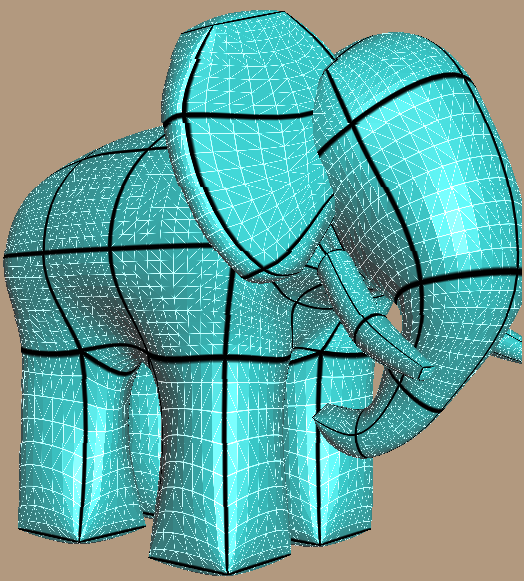
\includegraphics[width=0.5\textwidth]{gumbo_BezierByTess.png}
		\caption{Gumbo Bézier-Patch-Modell,	gerendert mit der Demo aus
			\url{http://prideout.net/blog/?p=49}: Je höher der Tessellation Level, desto mehr nähert
			sich die Geometrie der Form eines "`echten"', runden Bézier-Patches an}
		\label{fig:bezierByTess}
	\end{figure}
	
	Es handelt sich also um ein hardwarebeschleunigtes, für den Programmierer relativ einfach zu verwendendes
	Verfahren für dynamisches Level Of Detail (LOD). Somit lassen sich extreme Detail-Grade bei Nah-Aufnahmen
	erzeugen, ohne dass die Performance bei größerer Entfernung durch ein hochpolygonales Basis-Mesh leidet; 
	Für gewöhnlich hängt die Metrik zur LOD-Berechnung zumindest von der Entfernung der Geometrie zur Kamera,
	zuweilen auch von der Auflösung des zu rendernden Bildes, dem Kamera-Öffnungswinkel und weiteren Parametern ab.
	
	Abb. \ref{fig:gegenueberstellungTessNonTessCloseUpRaptorFoot} auf Seite 
	\pageref{fig:gegenueberstellungTessNonTessCloseUpRaptorFoot} demonstriert den Unterschied zwischen klassischer
	nicht-tessellierter Geometrie, und jener, auf die in Kombination mit Displacement Mapping das 
	Verfahren angewandt wurde.
	
	Um dieses Verfahren sinnvoll nutzen zu können, benötigt man als Asset erst einmal ein extrem detailliertes 3D-Modell.
	Zur Verwendung in dieser Arbeit wurde Das Raptor-Modell vom \emph{Digital Shape WorkBench} 
	\footnote{\url{http://shapes.aim-at-shape.net/view.php?id=178}} heruntergeladen
	und aufbereitet. Mit \emph{Meshlab} \footnote{\url{http://meshlab.sourceforge.net/}} wurde das
	zwei Millionen Dreiecke zählende Mesh schließlich auf 11000 Dreiecke, also fast um den Faktor 200
	reduziert.\\
	Mit \emph{Blender} wurden für das vereinfachte Modell Textur-Koordinaten erzeugt,
	dann durch Projektion des Originals auf das vereinfachte Modell
	eine Normal Map und eine Displacement Map gebaked.
	Hierbei handelt es sich um Texturen, die angeben, inwiefern sich ein Attribut der
	Original-Geometrie von der vereinfachten Geometrie in Richtung der Normale der vereinfachten 
	Geometrie unterscheidet. Im Falle der Normal Map
	handelt es sich um die Abweichung der Oberflächen-Normale, bei der Displacement Map um den
	Abstand der Original-Geometrie von der vereinfachten, siehe Abb. \ref{fig:normalDisp}. 
	Mithilfe dieser beiden Texturen lässt sich
	die Original-Geometrie aus der vereinfachten verlust-arm rekonstruieren, vorausgesetzt, die Maps
	liegen in genügend hoher Auflösung und Bit-Tiefe vor, und die Original-Geometrie hat keine "`Überhänge"'
	gegenüber dem einfachen Modell; sonst würde nämlich beim Baken mehr als ein Oberflächen-Element des Originals
	auf dieselbe Stelle auf dem simplen Mesh projeziert werden, was derselben Textur-Koordinate in den
	Maps entspräche, so zu Überschreibungen und Artefakten bei der Rekonstruktion führte.\\
	
	\begin{figure}[!h]
		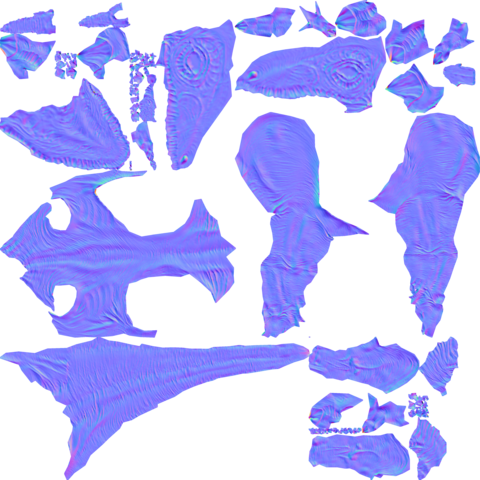
\includegraphics[width=0.5\textwidth]{resized/raptorNormThumb.png}
		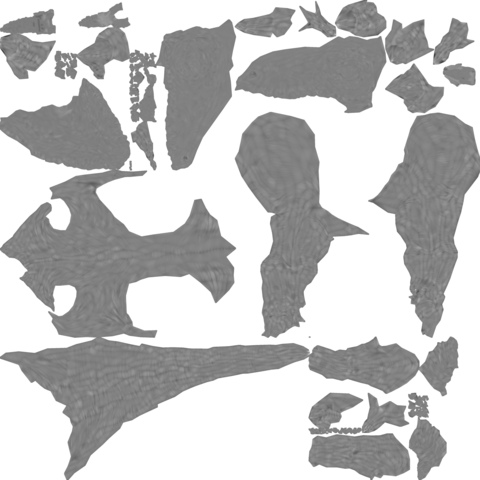
\includegraphics[width=0.5\textwidth]{resized/raptorDispThumb.jpg}
		\caption{Normal Map (links) und Displacement Map (rechts) des Raptor-Modells, im Original $4096^2$ Pixel
		mit 8 Bit Farbtiefe pro Kanal}
		\label{fig:normalDisp}
	\end{figure}
	
	Diese neue Repräsentation als vereinfachtes Mesh mit Normal und Displacement map kann nun
	von einem Echtzeit-Renderer, z.B. \emph{Flewnit} geladen werden. Ist keine OpenGL4-fähige Hardware vorhanden, 
	oder ist das Tessellation-Feature nicht erwünscht, kann das simple Modell klassisch gerendert werden,
	und Normal Mapping suggeriert geometrisches Detail, wo gar keines ist (siehe \ref{par:normalMapping}).
	Wird Tessellation jedoch unterstützt und erwünscht, werden zwei neue Shader-Stages erzeugt,
	der sog. \emph{Tessellation Control Shader} und der \emph{TessellationEvaluation Shader}.
	Diese beiden Stages folgen direkt auf den Vertex Shader, und kommen somit vor dem  Geometry
	und Fragment Shader.\\
	
	Jeder der beiden Tessellation Shaders wird pro \emph{Patch}-Vertex aufgerufen. Der \emph{Patch}
	ist ein neuer Primitiv-Typ in OpenGL. Er ist vertexbasiert und repräsentiert das, was sich
	an Semenatik einer bestimmten Menge von Vertices zuweisen lässt: ein schlichtes Dreieck, ein Viereck,
	oder aber die 16 Kontrollpunkte eines kubischen Bézier-Patches (s. Abb. \ref{fig:bezierByTess}), oder beliebige 
	weitere implizite oder explizite Oberflächen-Beschreibungen.

	
	Doch egal wie ein Patch für den Tessellation Control Shader aufgebaut ist, der Tessellator
	(die nicht-programmierbare Hardware-Einheit, welche die Geometrie nach der Tess. Control Stage
	erzeugt) produziert nur Drei- oder Vier-Ecke. Sobald man also mehr als vier Vertices pro Patch hat,
	stellt mindestens einer eine Form von Kontrollpunkt dar, der also nicht direkt einem "`klassischen"'
	Vertex entspricht.
	Wie viele und nach welchem Schema der Tessellator Primitive erzeugt, wird durch die
	Array-Variablen \lstinline|gl_TessLevelOuter| und \lstinline|gl_TessLevelInner| delegiert.
	Erstere Variable gibt pro Array-Element an, wie sehr die entsprechende Kante des Basis-Drei- bzw.
	Vierecks unterteilt werden soll. Letztere definiert, in wie viele Primitive der innere Bereich des
	Basis-Primitivs zerlegt werden soll. Die OpenGL-Implementation stellt sicher, dass die inneren und äußeren
	Tessellierungs-Levels sinnvoll miteinander verknüpft werden, so dass valide, zusammenhängende
	Primitive generiert werden. \\
	Je nach Typ des Basis-Primitivs, welches tesselliert wird sind die \lstinline|gl_TessLevel...|
	nur für bestimmte Längen definiert: Ein Dreieck hat. z.B. drei äußere Levels, pro Kante einen,
	und einen inneren. Ein Viereck hat jeweils einen Tessellation Level mehr, beim inneren also einen Level pro Achse.
	Dass man vor allem die Tessellation Levels für die Kanten des Basis-Primitivs einzeln bestimmten kann,
	ist sehr wichtig zur Vermeidung von  Unstetigkeiten zwischen benachbarten Patches. Hier sollten gemeinsame Kanten
	auch den selben Tessellation Level bekommen, damit die Kanten nicht "`aufbrechen"', indem Vertices der tessellierten
	Primitive nicht mehr benachbart sind.\\
	Dadurch, dass die Tessellation Levels nicht 1:1 mit der Anzahl an Vertices assoziiert sind, sollte immer nur
	ein bestimmter Vertex sich für das Schreiben eines bestimmten Tessellation Levels verantwortlich fühlen.
	Teilweise spielen für diese Berechnungen auch die Ergebnisse der anderen Vertices im Patch eine Rolle;
	Diese Ergebnisse sind für alle Vertices im Patch lesbar, sofern in eine (built-in oder selbst definierte
	per-Vertex oder per-Patch)	Output-Variable geschrieben wurde, und anschließend 
	\lstinline[language=GLSL]|barrier()| aufgerufen wurde.
	
	In \emph{Flewnit} ist zur Zeit nur der Patch-Typ mit drei Vertices, der genau ein Dreieck repräsentiert,
	unterstützt. Der Mehrwert an geometrischem Detail wird wie erwähnt durch Displacement Mapping
	im Tess. Evaluation Shader erzeugt. Die Anzahl an Vertices pro Patch lässt sich über die
	Routine \lstinline|glPatchParameteri(GL_PATCH_VERTICES, numVerticesPerPatch)| definieren.\\
	
	
	Der Hauptzweck des Tessellation Control Shaders ist also, die Tessellation Levels zu bestimmen.
	Außerdem, um einen weichen Übergang vom flachen Basis-Primitiv zum plastischen Relief der voll tessellierten
	und verschobenen Geometrie zu erreichen, wird in meiner LOD-Implementaion noch pro Vertex ein 
	\lstinline|distanceDependentDisplacementFactor| vom Control- an den Evaluation Shader übergeben, der einen 
	Gewichtungsfaktor zwischen 0 und 1 darstellt. In einem bestimmten Enfernungs-Intervall von der Betrachter-Kamera nimmt 
	der Displacement-Faktor zu. Wäre dies nicht der Fall, würden selbst die Vertices des Detail-armen, 
	nicht tessellierten Modells, immer gemäß der Displacement Map verschoben werden. Dies hätte 
	unschöne Artefakte durch Undersampling der Displacement Map zur Folge. 
	Dieser Wert errechnet sich wie folgt:
	\begin{lstlisting}[language=GLSL]
float calculateDistanceDependentLODFactor( float distanceVS )
{
 //distanceVS > distanceToBeginWithTesselation --> 0
 //distanceVS < distanceUntilFullSubdivision   --> 1
 //inbetween --> grow fast when far away (user doesnt notice becaus of distance), 
 //				 grow slower when coming closer
 //				 ==>> square root function in [0..1] satisfies these conditions
 float distFraction = 
    clamp(
      (distanceVS - distanceUntilFullSubdivision) / (distanceToBeginWithTesselation - distanceUntilFullSubdivision),
      0.0,
      1.0 
    );
 return 1.0- (sqrt(distFraction));
}
	\end{lstlisting}
	Diese Funktion ist rein experimentell entstanden. Eine weitere Option, um störende "Popping"-Artefakte
	zu vermeiden, ist, die Tessellierungs-Methode auf eine Form von "`fractional spacing"' zu stellen,
	z.B. über den Befehl \lstinline|layout(triangles, fractional_odd_spacing, ccw) in;| im Tess. Evaluation Shader:
	Diese Option bewirkt, dass mit steigenem Tessellation Level (es handelt sich um FLießkomma-Werte)
	entlang der Primitiv-Kanten von außen "`neue Vertices nachwachsen"'; beim "`equal spacing"' bleiben die
	Vertices des aktuellen Tesellation Levels an einem festen Ort innerhalb des Primitivs, bis ein
	Tessellation Level erreicht ist, der neue Vertices in die bestehenden "`zwischen streut"'. Somit
	"`poppen"' neue Vertices aus dem Nichts dazu, die auch noch ensprechend der oberen Funktion sofort displaced werden.\\
	
	Die Tessellation Levels der Dreiecks- Kanten, also die äußeren Tess-Levels, 
	orientieren sich an der Tessellation-Level-Berechnung im 
	DirectX 11- Spiel "`Metro 2033"', siehe \cite{tessMetro2033}, Folie 35:
	\begin{lstlisting}[language=GLSL]
float distanceFactor = calculateDistanceDependentLODFactor( edgeDistVS ) 
gl_TessLevelOuter[gl_InvocationID] =  
 clamp(	edgeLengthVS 
      	* numScreenPixels 
      	* tessQualityFactor 
      	* distanceFactor,
      minTessLevel, maxTessLevel );   
	\end{lstlisting}
	\lstinline|minTessLevel| und \lstinline|maxTessLevel| sind benutzerdefinierte uniform Variablen,
	die vermeiden sollen, dass ein Objekt komplett verschwindet 
	(Tess. Level 0 heißt, dass gar kein Primitiv erzeugt wird), bzw. dass der Tess. Level einen benutzerdefinierten 	
	Grenzwert nicht überschreiten darf.
	Der \lstinline|tessQualityFactor| ist ebenso eine benutzerdefinierbare Uniform Variable. 
	\lstinline|edgeLengthVS| gibt die Länge der Kante im Viewspace an. Hier sei explizit erwähnt, dass die Tessellation-
	Parameter invariant zur Kamera-Orientierung sein müssen, da es sonst bei Rotationen wieder zu störenden
	"`Popping-Artefakten"' kommt. Daher müssen wir im View- oder Worldspace rechnen, selbst wenn dann bei Primitiven,
	die in einem spitzen Winkel betrachtet werden, für die Bildqualität eines spezifischen Renderings eigentlich
	unnötig hohe Tesellation Levels generiert werden.
	Das LOD in \emph{Flewnit} weicht insofern von der in Metro 2033 verwendeten Formel ab, dass nicht durch
	die Distanz der Kantenmitte zur Betrachter-Kamera dividiert wird, sondern mit dem Wert multipliziert wird,
	der durch \lstinline|calculateDistanceDependentLODFactor(edgeDistVS)| errechnet wird.
	Somit ergibt sich eine bessere Kontrolle über den Bereich, in dem das Morphing zwischen niedrigstem
	und höchsten Tessellierungs- und Displacement- Faktor stattfinden soll.\\
	
	Schließlich, nach der Primitiv-Erzeugung durch den Tessellator, wird der Tessellation Evalutaion Shader
	pro generierten Vertex aufgerufen. Wieder stehen alle Eingangs-Patch-Vertices zur Verfügung.
	Bei Dreicks-Tessellierung sind die Primitiv-relativen Koordinaten eines Vertices im Tess- Eval. Shader
	baryzentrische Koordinaten. Die Viewspace-Attribute eines generierten Vertex lassen sich also einfacher
	(zunächst einmal ohne Displacement Mapping) bestimmen durch das Makro:
	\begin{lstlisting}[language=GLSL]
	 #define BARYCENTRIC_WEIGHTED(var) ( gl_TessCoord.x * input[0].var + gl_TessCoord.y * input[1].var + gl_TessCoord.z * input[2].var )
	\end{lstlisting}
	\lstinline|input| ist der Interface-Block, durch den benutzerdefinierte Variablen von einer Shader Stage zur nächsten
	weitergegeben werden 
	\footnote{Ein solches Shader-Interface ist nicht zu verwechseln mit einem \lstinline|struct|. 
	Interface-Block-Definitionen in GLSL vermeiden Namens-Konflikte zwischen gleichartigen input- und output-Variablen 
	einer Stage; Dieser Umstand macht das Parameter-Durchreichen bedeutend unkomplizierter; 
	Doch dieses Feature wird in dieser Ausarbeitung nicht detaillierter behandelt, 
	da es mit den Algorithmen als solchen nicht viel zu tun hat}.
	Die geometrischen Attribute werden also wie folgt gesetzt:
	\begin{lstlisting}[language=GLSL]
output.position =   BARYCENTRIC_WEIGHTED(position);
output.normal   =   BARYCENTRIC_WEIGHTED(normal);

  output.tangent =  BARYCENTRIC_WEIGHTED(tangent);

output.texCoords =  BARYCENTRIC_WEIGHTED(texCoords);
	\end{lstlisting}
	
	Das Displacement Mapping wird angewandt, indem die berechneten Textur-Koordinaten zum Lookup
	der Displacement Map per \lstinline|texelfetch(..)| genutzt wird (automatisch gefilterter Textur-Lookup ist nur
	im Fragment Shader verfügbar).
	Um diesen Wert, skaliert mit einem benutzerdefinierten Faktor (der durchaus angebracht sein kann, wenn die
	Displacement Map aufgrund der niedrigen Bit-Auflösung unpassend skaliert ist) und dem gewichteten
	\lstinline|distanceDependentDisplacementFactor| aus der Control Stage, wird die Vertex-Position shcließlich entlang 
	ihrer normalisierten Normale verschoben:
	
	\begin{lstlisting}[language=GLSL]  
float displacementVal = 
  (
    texelFetch(
      displacementMap, 
      texelPos,
      0  //mip map level 0; not thought about sophisticated mip map usage in this context yet
    ).x 
    //note: when applying shift,scale and type conversion from uint to int and setting the texture parameters accordingly,
    //we could omit the following two operations: TODO test it
    -0.5 //normalized values: shift from [0..1] to [-0.5 .. +0.5]
  )
  *2.0 //scale from [-0.5 .. +0.5] to [-1..+1]
  ;
        
float weightedDistanceDependentDisplacementFactor = 
  BARYCENTRIC_WEIGHTED(distanceDependentDisplacementFactor);         

output.position +=  
  normalize(output.normal) * 
  displacementVal *
  displacementIntensity * 
  weightedDistanceDependentDisplacementFactor
  ;
	\end{lstlisting}
	Man bemerke, dass durch die baryzentrische Gewichtung des \lstinline|distanceDependentDisplacementFactor|
	für jeden Vertex, der auf einer Kante des Basis-Primitivs liegt, immer derselbe Dasplacement- Faktor bestimmt wird, 
	unabhänging zu welchem Patch er gerade gehört. Dies gilt allerding nicht für Patch-Kanten, wo auch
	sog. Seams, also Ränder der Textur-Koordinaten-Inseln (vgl. Abb. \ref{fig:normalDisp}), vorliegen, und die Displacement
	map nicht optimal (also mit Überlappungen, die über die UV-Inseln hinausgehen) gebaked ist.
	Leider zeigt meine zuletzt gebakte Displacement Map diese Seams. Es fehlt mir noch an Routine im Umgang mit Blender.
	Innerhalb der UV-Inseln sorgt jedoch das vorgestellte LOD für weiche Übergänge zwischen verschiedenen Patches.

	
\subsubsection{Implementierte Effekte}
	\label{sec:genericVisualEffects}
	Neben der Beleuchtung mit belibig vielen Point- und Spot Lights und dem oben vorgestellten LOD per Tessellation
	wurden noch Shadow Mapping, Normal Mapping und Environment Mapping implementiert. 
	Diese schon seit mehreren Jahren zum Standard- Feature-Set einer Graphik-Engine gehörenden Effekte
	sollen im Folgenden kurz vorgeststellt werden.
	

	\paragraph{Shadow Mapping}
	
	\paragraph{Normal Mapping}
	\label{par:normalMapping}
	
		
	\paragraph{Environment Mapping}


%%-------------------------------------------------------------------------------------------------------
\todo[color=green]{diesen klumbatsch in form bringen, mit bildern anreichern etc pp}

Zunächst zum Begriff "Mapping", der so oft auftaucht: Englisch "map"-"Landkarte", "to map"-"abbilden" Bedeutet in der Computergrafik meist die Abbildung eines Bildes auf eine Oberfläche nach einem bestimmten Algorithmus;

- Beleuchtung durch beliebig viele Punkt- und Spot-Lichtquellen (also Lichtquellen mit eineme gerichteten Kegel, Scheinwerfer)

- Shadow Mapping: Erzeugen eines bildes aus Tiefenwerten, anschließend vergleich der Tiefenwerte aus Kamerasicht mit denen aus Lichtquellensicht (der "shadow map", Schattenkarte), pixel im finalen Bild gilt als verdeckt wenn Tiefenwert aus Kamerasicht größer als der entsprechende Pixel in der shadow map, unverdeckt wenn nicht;

- Normal Mapping: Verzerrung der Oberflächen-Normalen (Vektor Sekrecht zur Oberfläche) um relief-artige Geometriedetails zu simulieren, ohne dass tatsächlich diese feine Geometrie in der virtuellen Szene existiert; Dies spart Rechenleistung und Speicher im Vergelcih zu einer Szene, wo all dieses Detail tatächlich in der Geometrie vorhanden wäre; Anschauliches Anwendungsbeispiel: Illusion der feinen Geometrie von Rauhfasertapete auf einem schlichten Quadrat; Nachteil: Die geometrische Illusion brich bei flachen Betrachtungswinkeln ein, die Flachheit der eigentlichen, simplen Geometrie fällt dann auf; Die Information der verzerrten Normalen stammt ebenfall aus einem Bild, der "normal map"; Diesmal werden die Pixelwerte jedoch nicht als Farben oder Tiefenwerte, sondern als Abweichung von der unverzerrten Normalen interpretiert (rot->x-Achse;grün->y-Achse; blau->z-Achse); Da im Computer alles nur Zahlen sind und Semantik erst durch unsere Verwendung und Wahrnehmung erlangen, und da die Graphikkarten so weit flexibel/programmierbar geworden sind, dass man als Programmierer Kontrolle über derartige "Um-Interpretierung" hat, ist dies möglich;

- Environment mapping: Der Trick, perfekt spiegelnde Materialen vorzugaukeln: Es wird in einer "Cube map" nachgeschaut, einer Sammlung von sechs bildern, wo jedes Bild eine Würfelseite repräsentiert; Die Reichtung der Normalen eines Pixels wird umgerechnet in eine Koordinaten, mit der in der Cube Map nachgeschaut wird; Dieser Frabwert fießt dann in die Farbe des Pixels des finalen Bildes ein; Vorteil: Dinge wie lackierte Autokarosserien lassen sich ganz gut vorgaukeln, mit recht geringem Rechenaufwand; Nachteil: Da für gewöhnlich nur in einem statischen Bild nachgeschaut wird, können dynamische Änderungen der Szene bei der "pseudo-spiegelung" nicht erfasst werden; Ein Objekt, welches sich nache eines autos bewegt, bewegt sich ein seiner "Spiegelung" nicht; Aus solchen Gründen sind in Cube maps oft nur sehr entfernte Dinge dargestellt: Horizong, Himmel, Wolken etc.; Diese Dinge ändern sich in der Realistät ja nicht so schnell, daher fällt der Nachteil beim environment mapping unter dieser Einschränkung nicht mehr so drastisch auf; Der Hintergrund, die orangene Dämmerung, ist gnau diese Cube map, die ich also sowohl für die Pseudo-Spiegelung als auch als "Füllmaterial" dort, wo ich keine Geometrie in der Szene habe, verwende;

- Tesselation: Wie Bei Normal Mapping soll der wahrgenommene Detailgrad der Geometrie erhöht werden; Jedoch erzeugt die Tesselation "`echte"' Geometrie, in Abhängigkeit von der Entwerfnung eines Objekte zur Betracher-Kamera; Somit wird dort Geometrie erzeugt, wo sie nötig für den Detailgrad des aktuellen Bildes ist, und dort eingespart, wo sie momentan unnötig ist; Diese Technik hat nicht die Nachteile des Normal mappings; Jedoch Ist durch die Reine Erzeugung von Geometrie noch nicht viel gewonnen; Sinn bekommt diese neue  Geometrie wert dann, wenn sich auch wirklich mehr Datail mit ihr darstellen lässt; Erreicht wird dies durch eine sogenannte Displacement Map (frei Übersetzt "Verschiebungs-Karte", ein Bild, in dem Tiefenwerte der Hoch-detaillierten Geometrie gepeichert sind). Die neu erzeugte Geometrie wird also entlang der Normalen um den Betrag verschoben, wie in der Displacement Map eingetragen ist; Somit entsteht ein "tatsächliches Relief", im gegensatz zum Vorgegaukelten Relief beim Normal Mapping; MEhr Details erspare ich dir, z.b. Warum man Normal Mapping trotzdem immer noch für die Beleuchtung braucht, trotz der Tesselation und dem Displacement mapping;

Anmerkung: Weil ich Tesselation so toll finde, habe ich mir das Velociraptor-3D-Modell aus dem Internet besorgt; Dieses hatte 5 Milloonen Dreiecke; Ich habe es mit einem Programm (was ich nicht selbst geschrieben habe, davon versteh ich leider noch viel zu wenig) herunterrechnen lassen, so  dass ein vereinfachtes Modell mit etwa 11000 Dreicken entstand, also ein etwa zweitausend mal simpleres Modell. Mit einem anderen Programm habe ich dann die Geometrie des komplexen Modells auf die des simplen Modells projeziert, die detailgrad-bedingte Distanz zwischen den Geometrien in ein Bild geschrieben; Dieses Bild ist die Displacement map für die Tesselation izur Darstellung in meinem eigenen Programm; Somit kann ich nun den Dinosaurier beinahe so detailliert darstellen, wir er im Originalmodell vorliegt, jedoch mit viel höheren Bildwiederholungsraten; 

%%-------------------------------------------------------------------------------------------------------
	  

\clearpage
